\documentclass[9pt,landscape]{memoir}
\usepackage{multicol}
\usepackage{calc}
\usepackage{ifthen}
\usepackage[landscape]{geometry}
\usepackage{hyperref,siunitx}
\usepackage{amssymb,amsmath,verbatim,graphicx,enumitem,microtype,upquote,units,booktabs,siunitx,hyperref}

\ifthenelse{\lengthtest { \paperwidth = 11in}}
{ \geometry{top=.5in,left=.5in,right=.5in,bottom=.5in} }
{\ifthenelse{ \lengthtest{ \paperwidth = 297mm}}
    {\geometry{top=1cm,left=1cm,right=1cm,bottom=1cm} }
    {\geometry{top=1cm,left=1cm,right=1cm,bottom=1cm} }
}

% Turn off header and footer
\pagestyle{empty}
\renewcommand{\familydefault}{\sfdefault}
\setlist[itemize]{leftmargin=0pt, noitemsep, before={\vspace*{-.25\baselineskip}}, after={\vspace*{-\baselineskip}}}
\setlist[enumerate]{leftmargin=0pt, noitemsep, before={\vspace*{-.25\baselineskip}}, after={\vspace*{-\baselineskip}}}

% Redefine section commands to use less space
\makeatletter
\renewcommand{\section}{\@startsection{section}{1}{0mm}%
    {-1ex plus -.5ex minus -.2ex}%
    {0.5ex plus .2ex}%x
{\normalfont\large\bfseries}}
\renewcommand{\subsection}{\@startsection{subsection}{2}{0mm}%
    {-1explus -.5ex minus -.2ex}%
    {0.5ex plus .2ex}%
{\normalfont\normalsize\bfseries}}
\renewcommand{\subsubsection}{\@startsection{subsubsection}{3}{0mm}%
    {-1ex plus -.5ex minus -.2ex}%
    {1ex plus .2ex}%
{\normalfont\small\bfseries}}
\makeatother

% Define BibTeX command
\def\BibTeX{{\rm B\kern-.05em{\sc i\kern-.025em b}\kern-.08em
T\kern-.1667em\lower.7ex\hbox{E}\kern-.125emX}}

% Don't print section numbers
\setcounter{secnumdepth}{0}


\setlength{\parindent}{0pt}
\setlength{\parskip}{0pt plus 0.5ex}

\makeatletter
\newsavebox\myboxA
\newsavebox\myboxB
\newlength\mylenA

\newcommand*\xoverline[2][0.75]{%
    \sbox{\myboxA}{$\m@th#2$}%
    \setbox\myboxB\null% Phantom box
    \ht\myboxB=\ht\myboxA%
    \dp\myboxB=\dp\myboxA%
    \wd\myboxB=#1\wd\myboxA% Scale phantom
    \sbox\myboxB{$\m@th\overline{\copy\myboxB}$}%  Overlined phantom
    \setlength\mylenA{\the\wd\myboxA}%   calc width diff
    \addtolength\mylenA{-\the\wd\myboxB}%
    \ifdim\wd\myboxB<\wd\myboxA%
       \rlap{\hskip 0.5\mylenA\usebox\myboxB}{\usebox\myboxA}%
    \else
        \hskip -0.5\mylenA\rlap{\usebox\myboxA}{\hskip 0.5\mylenA\usebox\myboxB}%
    \fi}
\makeatother

\renewcommand{\hat}{\xoverline}

% -----------------------------------------------------------------------

\begin{document}

\raggedright
\footnotesize
\begin{multicols}{3}
    \section{One Factor Experiments}

            \begin{equation*}
                H_0 = \mu_1 = \ldots = \mu_1
            \end{equation*}

            \begin{equation*}
                H_1 = \text{two or more of the $\mu_i$ are different}
            \end{equation*}

            \begin{align*}
                SSTr &= \sum_{i = 1} ^I J_{i.} {(\bar{X}_{i.} - \bar{X}_{..})}^2 \\
                     &= \sum_{i = 1} ^I J_i \bar{X}_{i.}^2 - N \bar{X}_{..}^2
            \end{align*}

            \begin{align*}
                SSE &= \sum_{i = 1} ^I \sum_{j = 1} ^{J_i} {(X_{ij} - \bar{X}_i)}^2 \\
                    &= \sum _{i = 1} ^I \sum _{j = 1} ^{J_i} X_{ij} ^2 - \sum _{i = 1} ^I J_i \bar{X}_i ^2
            \end{align*}

            \begin{equation*}
                MSTr = \frac{SSTr}{I - 1} \qquad MSE = \frac{SSE}{N - I}
            \end{equation*}

            \begin{equation*}
                F = \frac{MSTr}{MSE}
            \end{equation*}

            \begin{equation*}
                SST = SSTr + SSE
            \end{equation*}

            \begin{align*}
                SST &= \sum _{i = 1} ^I \sum_{j = 1} ^{J_i} {(X_{ij} - \bar{X}_{..})}^2  \\
                    &= \sum _{i = 1} ^I \sum_{j = 1} ^{J_i} X_{ij} ^2 - N\bar{X}^2
            \end{align*}

            \begin{align*}
                p-\text{value} &< \alpha \implies \text{reject $H_0$} \\
                p-\text{value} &\geq \alpha \implies \text{fail to reject $H_0$}
            \end{align*}

    \section{Two Factor Experiments}
            \begin{align*}
                X_{ijk}        &= \mu + \alpha_i + \beta_j + \gamma_{ij} + \epsilon_{ijk} \\
                \alpha_i       &= \bar{\mu}_{i.} - \mu \\
                \beta_j        &= \bar{\mu}_{.j} - \mu \\
                \gamma_{ij}    &= \mu_{ij} - \bar{\mu}_i - \bar{\mu}_j + \mu \\
                \epsilon_{ijk} &= X_{ijk} - \mu_{ij}
            \end{align*}

            \begin{align*}
                H_{0, AB}: \gamma_{11} = \gamma_{12} = \cdots = \gamma_{IJ} = 0 \\
                H_{H, AB}: \text{at least one of the $\gamma_{ij}$ is nonzero}
            \end{align*}

            \begin{align*}
                H_{0, A}: \alpha_1 = \alpha_2 = \cdots = \alpha_I = 0 \\
                H_{1, A}: \text{at least one of the $\alpha_i$ is nonzero}
            \end{align*}

    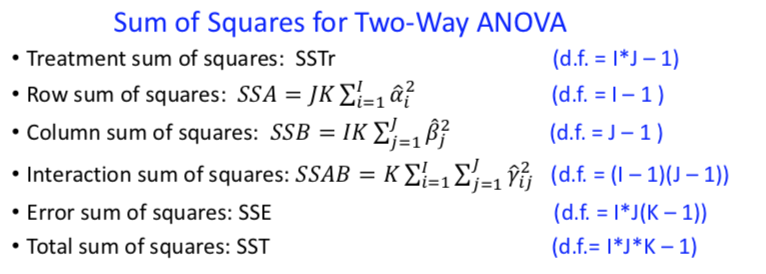
\includegraphics[width=.9\columnwidth]{degrees}

    \begin{equation*}
        F_{AB}^* = \frac{MSAB}{MSE} \qquad F_A ^* = \frac{MSA}{MSE} \qquad \frac{MSB}{MSE}
    \end{equation*}

    \begin{equation*}
        MSA = \frac{SSA}{I - 1} \qquad MSB = \frac{SSB}{J - 1} \qquad MSAB + \frac{SSAB}{(I - 1)(J - 1)}
    \end{equation*}

    \section{Bernoulli Distribution}
            \begin{align*}
                \mu_x    &= p \\
                \sigma_x ^2 &= p(1 - p)
            \end{align*}

    \section{Binomial Distribution}
    \begin{equation*}
        p(x) = P(X = x) = \begin{cases}
            {n \choose x} p^x {(1 - p)}^{n - x} & x = 0, 1, \ldots, n \\
            0 & \text{otherwise}
        \end{cases}
    \end{equation*}

    where ${n \choose k} = \frac{n!}{k!(n - k)!}$
            \begin{align*}
                \mu_x = np \\
                \sigma_x ^2 = np(1 - p)
            \end{align*}

            \begin{equation*}
                \hat{p} = \frac{\text{number of successes}}{\text{number of trials}} = \frac{X}{n}
            \end{equation*}

            \begin{equation*}
                \sigma_{\hat{p}} = \sqrt{Var(\hat{p)}} \approx \sqrt{\frac{\hat{p}(1 - \hat{p})}{n}}
            \end{equation*}

    \section{Poisson Distribution}
            \begin{equation*}
                p(x) = P(X = x) = \begin{cases}
                    \frac{e^{-\lambda}\lambda^x}{x!} & x = 0, 1, \ldots, n \\
                    0 & \text{otherwise}
                \end{cases}
            \end{equation*}

            \begin{equation*}
                \mu_x = \lambda \qquad \sigma_x ^2 = \lambda
            \end{equation*}

    \section{The Normal Distribution}
    If a continuous random variable $x$ with mean $\mu$ and variance $\sigma^2$ has the following probability density function

    \begin{equation*}
        f(x) = \frac{1}{\sigma \sqrt{2\pi}} e^{-\frac{{(x - \mu)}^2}{2\sigma^2}}
        \end{equation*}

        \begin{equation*}
            Z = \frac{X - \mu}{\sigma}
        \end{equation*}

        \section{The Exponential Distribution}
        The notation is as follows $X \textasciitilde Exp(\lambda)$

        \begin{equation*}
            f(x) = \begin{cases}
                \lambda e^{-\lambda x} & x = 0, 1, \ldots, n \\
                0 & \text{otherwise}
            \end{cases}
        \end{equation*}

                \begin{equation*}
                    F(x) = \begin{cases}
                        0 & x \leq 0 \\
                        1 - e^{-\lambda x} & x > 0
                    \end{cases}
                \end{equation*}

                \begin{equation*}
                    P(T > t + s | T > s) = P(T > t)
                \end{equation*}

        \begin{equation*}
            s_i ^2 = \sigma_i ^2 = \frac{1}{J_i - 1} \sum _{j = 1} ^{J_i} {\left( X_{ij} - \bar{X_{i.}} \right)}^2
        \end{equation*}
    \end{multicols}
    \end{document}
